\documentclass[11pt]{beamer}

\usetheme{metropolis}

\usepackage{graphicx}
\usepackage{physics}
\usepackage{adjustbox}
\usepackage{caption}
\usepackage{chemformula}
\usepackage{quoting}
\usepackage[style=chem-angew,backend=bibtex]{biblatex}
\bibliography{references}
%
% Choose how your presentation looks.
%
% For more themes, color themes and font themes, see:
% http://deic.uab.es/~iblanes/beamer_gallery/index_by_theme.html
%
\mode<presentation>
{
  \usetheme{default}      % or try Darmstadt, Madrid, Warsaw, ...
  \usecolortheme{default} % or try albatross, beaver, crane, ...
  \usefonttheme{default}  % or try serif, structurebold, ...
  \setbeamertemplate{navigation symbols}{}
  \setbeamertemplate{caption}[numbered]
  \setbeamerfont{footnote}{size=\tiny}
} 

\usepackage[english]{babel}
\usepackage[utf8]{inputenc}
\graphicspath{{image/}}

\AtBeginSection[]{
\begin{frame}{Outline}
  \tableofcontents[currentsection]
\end{frame}
}

\title{Chapter 9: Gaseous State}
\institute{Chemistry Department, Cypress College}
\date{Nov 28, 2022}

\begin{document}

\begin{frame}
  \titlepage
\end{frame}

\begin{frame}{Class Announcements}
  \textbf{Lab}
  \begin{itemize}
  \item Lab Practicuum Week; Mon - Lab Review
  \item Submit \textbf{All} Lab Assignments...
  \end{itemize}

  \textbf{Lecture}
  \begin{itemize}
  \item Finish up Ch 9; Begin Ch 10 and 11
  \item Final Exam Dec 10th in Lecture
  \item Quiz and Homework posted this Fri, Dec 2nd
  \end{itemize}
\end{frame}

\section{Review: Ideal Gas Law}

\begin{frame}{Greenhouse Effect}
  \centering
  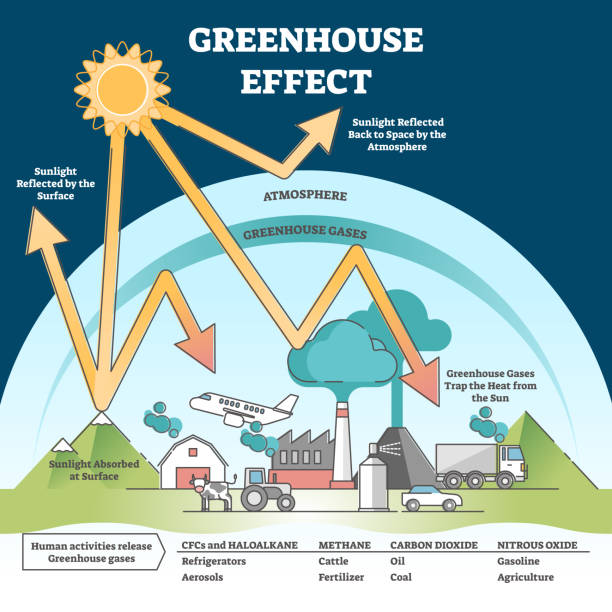
\includegraphics[width=\linewidth]{greenhouse_effect}
\end{frame}

\begin{frame}{Recall the Models}
  \textbf{Plum Pudding Model}
  \centering
  
  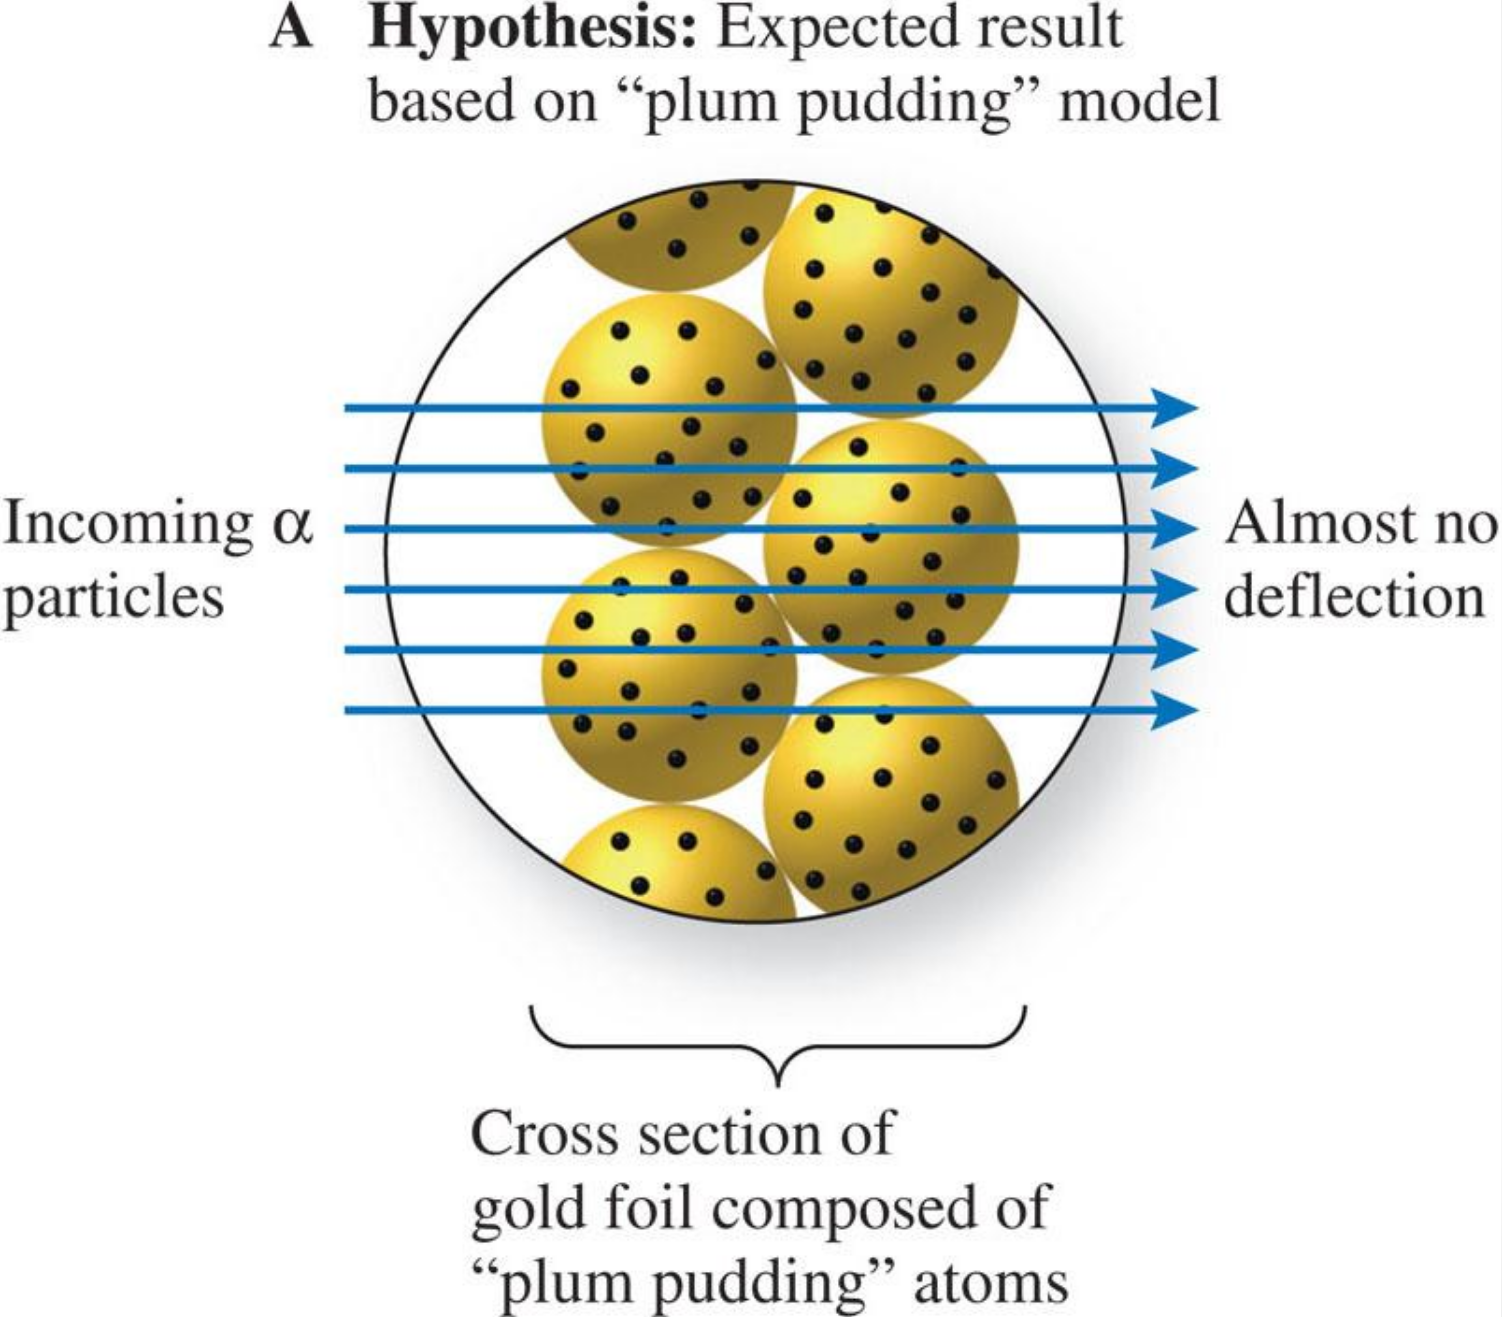
\includegraphics[width=0.7\linewidth]{test_hypothesis}
\end{frame}

\begin{frame}{Recall the Models}
  \centering
  \textbf{Bohr Model}

  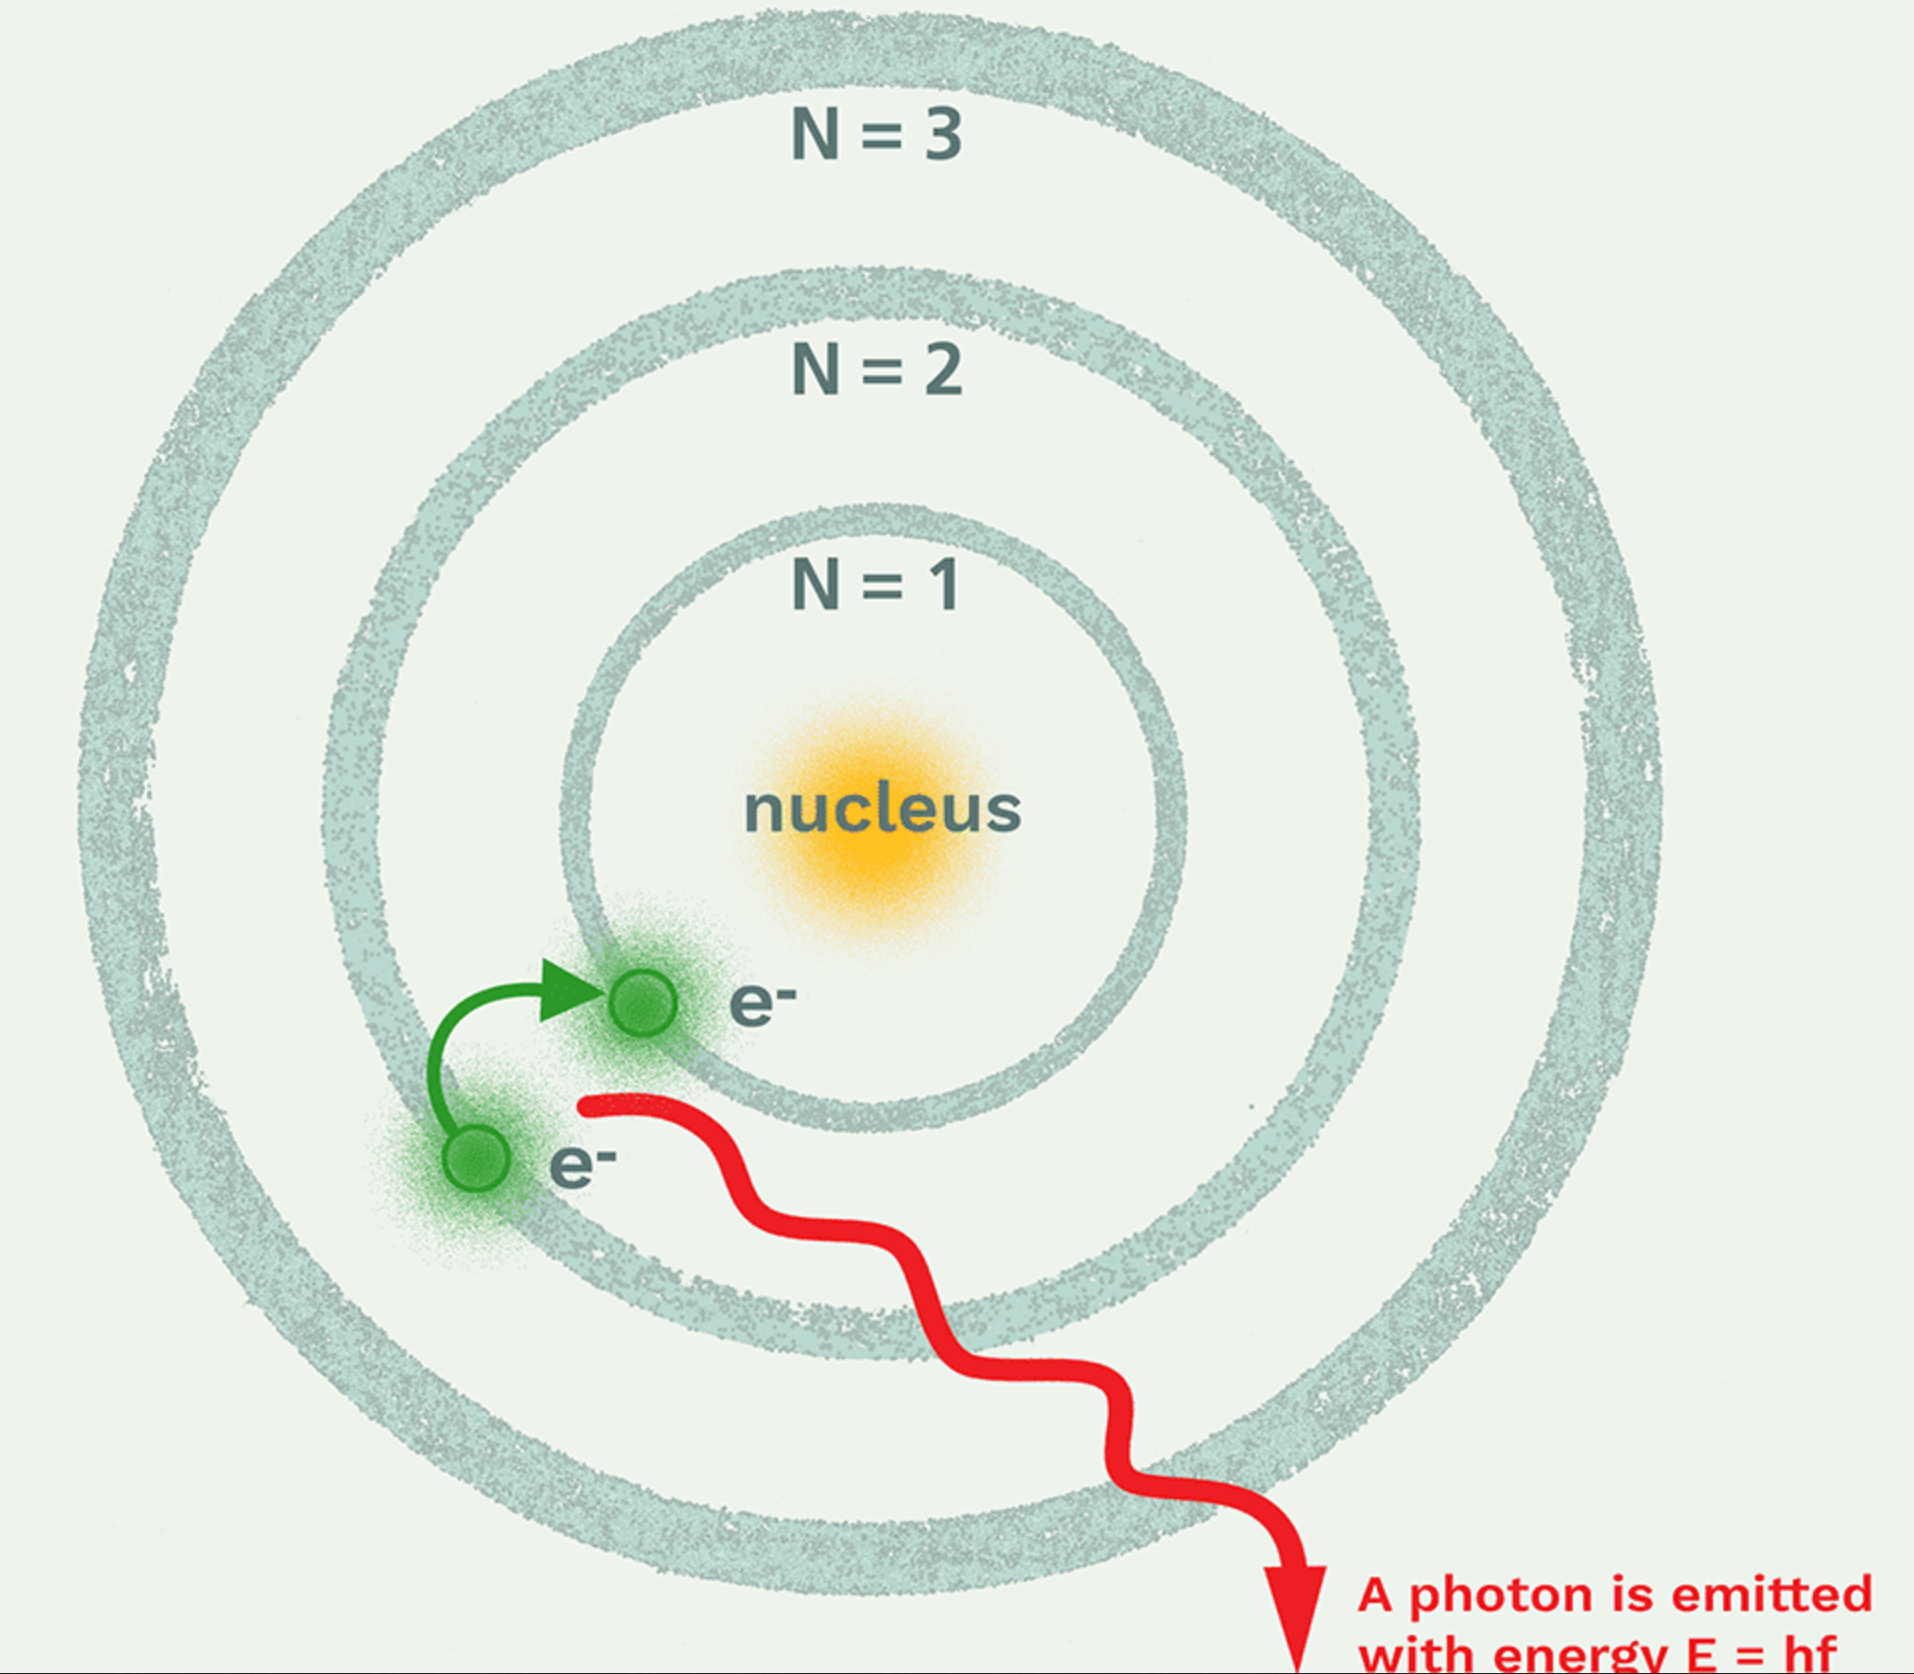
\includegraphics[width=0.7\linewidth]{bohr_model}
\end{frame}

\begin{frame}{Ideal Gas Model}
  \textbf{Assumptions}
  \begin{itemize}
  \item There is a large number of molecules that are
    in random motion
  \item Volume of the molecule is small relative to the volume occupied
    by the gas
  \item All molecules of a given gas are identical
  \item There no interactions between molecules (intermolecular forces)
  \item Collisions between gas molecules are perfectly elastic
  \end{itemize}
\end{frame}

\begin{frame}{Ideal Gas Formula}
  \begin{equation}
    PV = nRT
  \end{equation}
  where $P$ is pressure (atm), $V$ is volume (L), $n$ moles of gas (mols),
  $R$ is gas constant, and $T$ is temperature (K)

  \onslide<2->{\textbf{Gas Constants} - Use the appropriate once based on the
  units in the problem
  \begin{align}
    R = & 8,314.46\,\frac{\text{L Pa}}{\text{K mol}}
    = 0.082057\,\frac{\text{L atm}}{\text{K mol}} \nonumber\\
    = & 62.3636\,\frac{\text{L Torr}}{\text{K mol}} \nonumber
  \end{align}
  }
\end{frame}

\begin{frame}{Using Ideal Gas to Obtain Gas Laws}
  \textbf{Boyle's Law} - hold $n$ and $T$ constant
  \onslide<2->{\begin{align}
    PV = & nRT \nonumber \\
    PV = & \text{constant} \\
    P_1V_1 = & P_2V_2 \nonumber
    \end{align}
  }
  \onslide<3->{\textbf{Charles' Law} - hold $n$ and $P$ constant}
  \onslide<4->{\begin{align}
    PV = & nRT \nonumber \\
    \frac{V}{T} = & \frac{nR}{P} = \text{constant} \\
    \frac{V_1}{T_1} = & \frac{V_2}{T_2} \nonumber
    \end{align}
  }
\end{frame}

\begin{frame}{Finding Density from Ideal Gas Law}
  \textbf{Q:} What are the units for density?
  \onslide<2->{\begin{align*}
      PV = & nRT \\
      \frac{n}{V} = & \frac{P}{RT}
    \end{align*}
    Given this ratio, the last step is to multiply by the molar
    mass of the given substance
    \begin{align*}
      D = \frac{n\,MM}{RT}
    \end{align*}
    where $MM$ is the molar mass
  }
\end{frame}

\begin{frame}{Finding Molar Mass from Ideal Gas Law}
  \textbf{Q:} What are the units for molar mass?
  \onslide<2->{\begin{align*}
      PV = & nRT \\
      n = & \frac{PV}{RT}
    \end{align*}
    Determine the moles and given the mass, divide by the moles
  }
\end{frame}

\section{Dalton's Law of Partial Pressures}

\begin{frame}{Dalton's Law of Partial Pressures}
  Gases in a mixture behave independently and exert the same pressure they would
  exert if they were in a container alone
  \begin{equation}
    P_\text{Total} = P_A + P_B + P_C + \cdots
  \end{equation}
  where $P_\text{Total}$ is the total pressure and $P_A, P_B, \cdots$ are the
  pressures of the components
\end{frame}

\begin{frame}{Dalton's Law of Partial Pressures}
  \begin{center}
    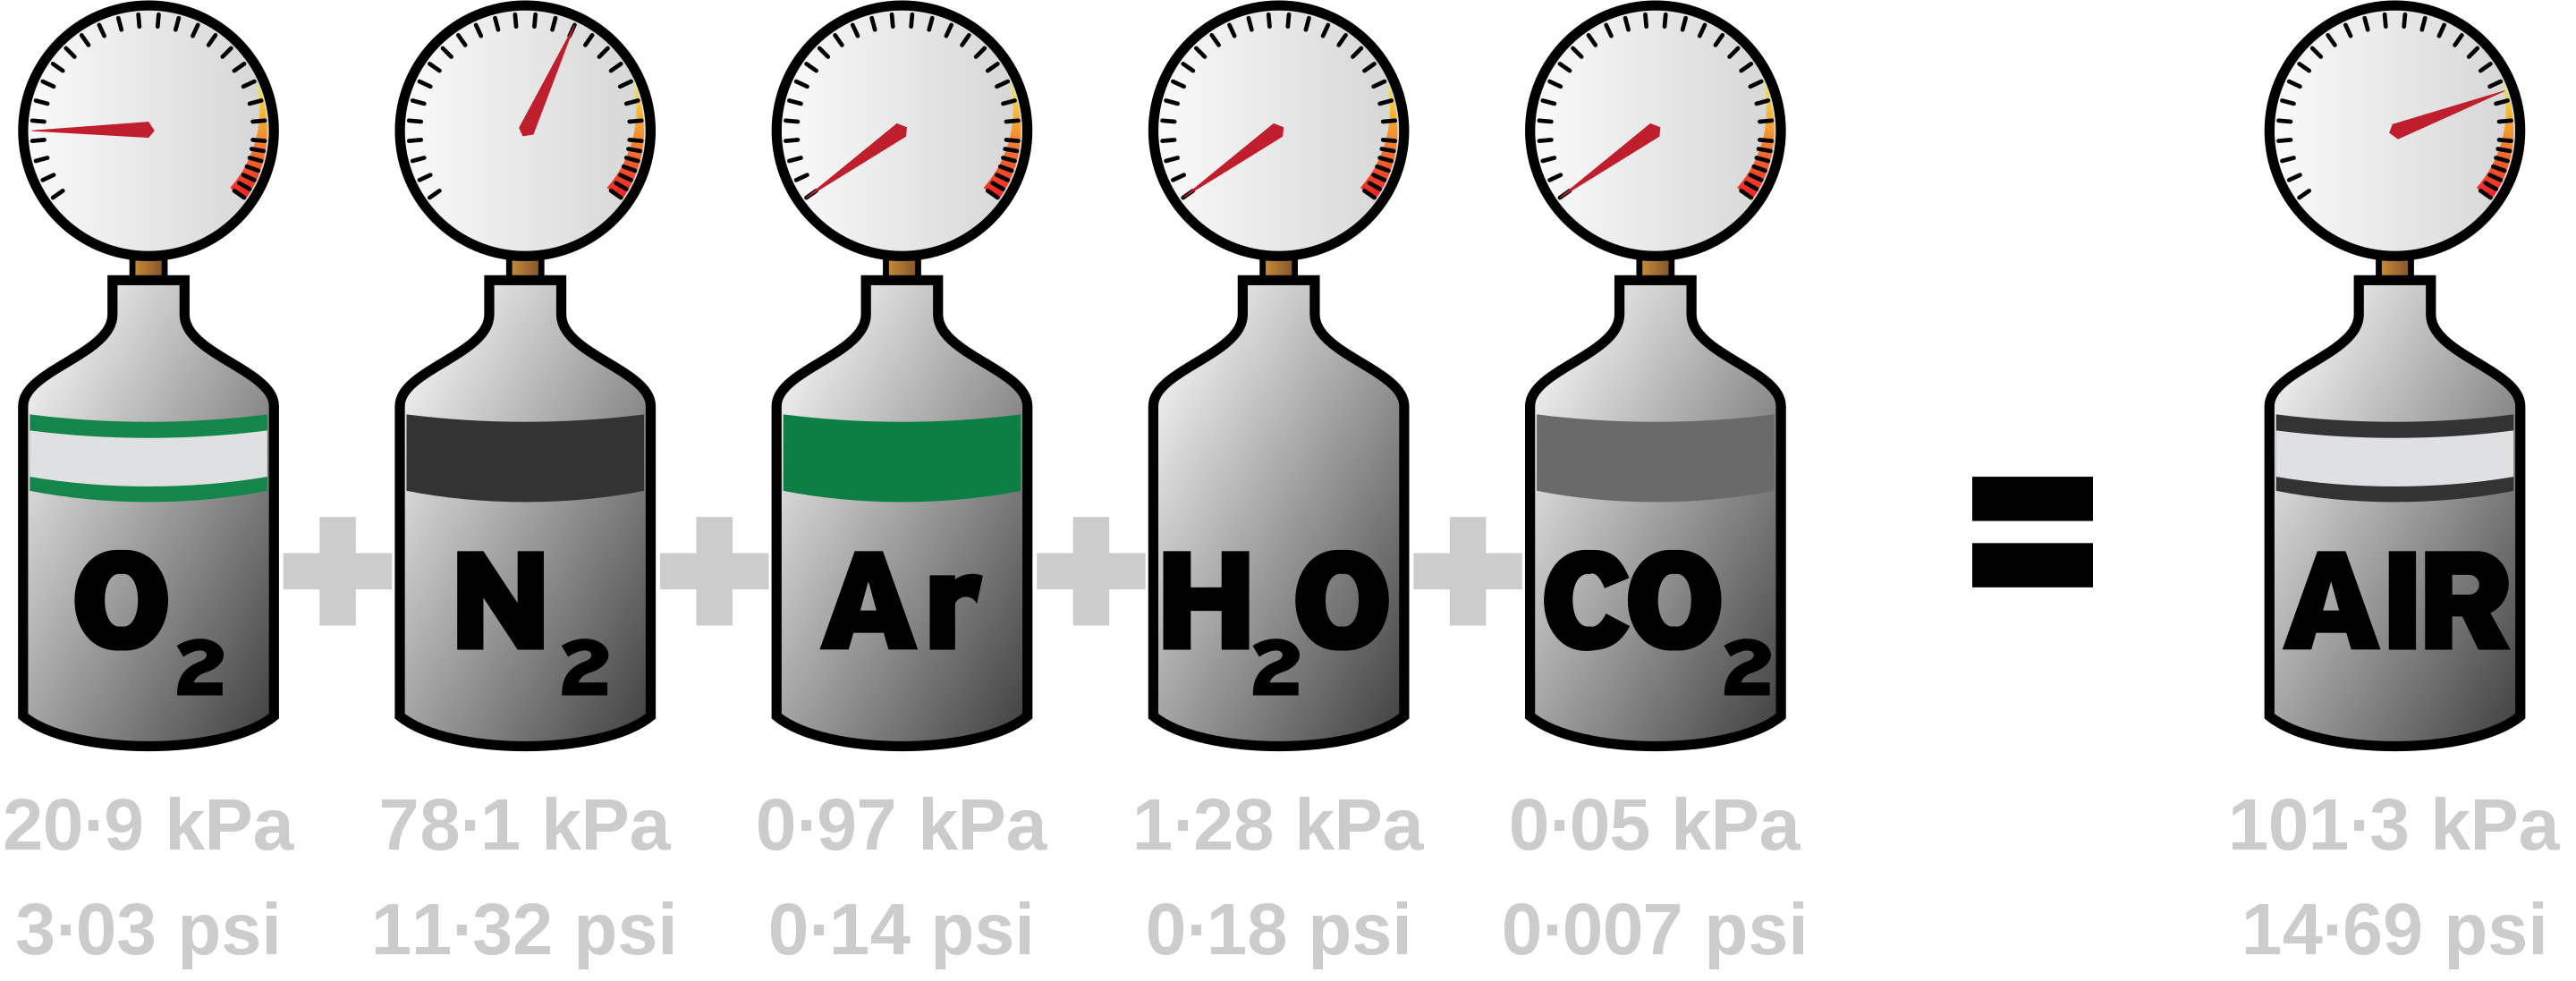
\includegraphics[width=\linewidth]{dalton_partial}
  \end{center}
  \begin{equation}
    P_\text{Total} = P_\text{O2} + P_\text{N2} + P_\text{Ar}
    + P_\text{H2O} + P_\text{CO2}
    \nonumber
  \end{equation}
\end{frame}

\begin{frame}{Practice: Dalton's Law of Partial Pressure}
  Suppose gaseous oxygen (O$_2$) is produced by:

  2KClO$_3$(s) $\rightarrow$ 2KCl(s) + 3O$_2$(g)

  If 1.50L of O$_2$ is collected over water at 300.K and 0.970atm,
  how many moles of O$_2$ is produced? The vapor pressure of water
  is 0.0351atm.
  \vspace{1.3in}
\end{frame}

\begin{frame}{Mole Fraction}
  Expressing the relative amounts of substances in a mixture
  \begin{equation}
    \chi_A = \frac{n_A}{n_\text{Total}}
  \end{equation}
  where $\chi_A$ is the mole fraction of component A, $n_A$ is the
  amount of moles for A, and $n_\text{Total}$ is the total amount of
  moles in the mixture
\end{frame}

\begin{frame}{Dalton's Law of Partial Pressure}
  Since each gas component exert its own pressure, the partial pressure
  of each component can be expressed by
  \begin{equation}
    P_A = \chi_A P_\text{Total} = \frac{n_A}{n_\text{Total}} P_\text{Total}
  \end{equation}
\end{frame}

\begin{frame}{Practice: Dalton's Law of Partial Pressures}
  A flask contains a mixture of 1.25 mols of hydrogen gas and 2.90 moles
  of oxygen gas. If the total pressure is 104.kPa, what is the partial
  pressure of each gas?
  \vspace{1.5in}
\end{frame}

\section{Take it further: Combined with Chemical Reactions}

\begin{frame}{Practice: Moles-Volume}
  Assuming ideal gas conditions, the sample of H$_2$(g) occupies a 8.00L
  container at 5.00 atm and 298.15K. What volume of H$_2$O(g) is produced
  by the reaction at 423.15K and 0.947atm, if all H$_2$(g) reacts with
  copper(II) oxide?
  \vspace{1.5in}
\end{frame}

\begin{frame}{Practice: Mass-Volume}
  Assuming ideal gas conditions, how many moles CaCO$_3$(s) form if 3.45L of
  CO$_2$(g), measured at 318.15K and 1.37atm, react with excess CaO(s)? How
  many grams?
  \vspace{1.5in}
\end{frame}

\end{document}
